\documentclass[12]{article}
\usepackage{graphicx}
\usepackage{color}
\usepackage{algorithmic}
\usepackage{underscore}
\begin{document}

\title{\textbf{
\includegraphics[scale=0.5]{42.png}
\textcolor{red}{Universitatea din Craiova \\Facultatea de Automatic\u{a},Calculatoare \c{s}i Electronic\u{a}}}}
\date{\textbf{01 June 2018}}
\maketitle
\begin{center}

\includegraphics[scale=0.3]{cmp.jpg}
\end{center}
\textbf{Project : Algorithm Design} \\
\textbf{Title : Change Making Problem}\\
\textbf{Teachers : B\u{a}dic\u{a} Costin \& Murare\c{t}u Ionu\c{t} \& Becheru Alex} \\
\textbf{Student : Moraru Teodor Valentin} \\
\textbf{Section : Calculatoare Rom\^{a}n\u{a}\\ Year I\\ Group : 1.2 B}
\newpage
\tableofcontents

\newpage
\section{Problem Statement}

\textcolor{white}{}
\subsection{Title}
\textcolor{blue}  {A project designed to solve the Change Making Problem in two different methods : a greedy algorithm and a dynamic algorithm.}

\subsection{Description}
\textcolor{white}{}


My project target is to solve the change making problem in two different implementations .The owed sum , number of coins and the actual coins values are read  form the file "input.txt".The values in the file will be added by the uses as following : the first number in the file represents the owed sum , the second one is the number of coins and the others will be the coin values .

Dynamic allocation is the automatic allocation of memory in C/C++, Unlike declarations, which load data onto the programs data segment, dynamic allocation creates new usable space on the programs STACK(an area of RAM specifically allocated to that program).For this reason the matrix was dynamically allocated in the dynamic implementation.

The greedy method was kept as simple as possible in order to hit it's main target that of being an easy comprehensive code .But it is not as effective nor as 

\newpage
\section{Pseudocode}
\subsection{get_value}
\begin{algorithmic}[1]
\STATE get_value($INT$ *owed , $INT$ *coins_no , $INT$ coins_list[100])
\STATE $START$
\STATE $INT$ \ i , hold_owed ,hold_no
\STATE $FILE  *input\_file$
\STATE $input\_file=fopen("input.txt","r")$
\STATE $fscanf( input\_file,"\%d",\&hold\_owed)$
\STATE $*owed = hold_owed;$
\STATE $fscanf( input_file,"\%d",\&hold\_no)$
\STATE $*coins\_no = hold\_no$
\FOR {$i = 0$ \TO coins_no}
\STATE $fscanf( input_file, "\%d", \&coins\_list[i] )$
\ENDFOR
\STATE $fclose(input\_file)$
\STATE $END$
\end{algorithmic}


\subsection{greedy_method}
\begin{algorithmic}[1]
\STATE greedy_method($INT$ owed ,$INT$ coins_no ,$INT$ coins_list[100],$INT$ good_picks[100])
\STATE $START$
\STATE $INT$ \ i , good_picks[100]
\FOR {$i = 0$ \TO coins_no}
\STATE good_picks[i] = owed div coins_list[i]
\STATE owed = owed mod coins_list[i]
\ENDFOR
\IF{$(owed == 0)$}
\STATE print("Coins used:")
\FOR{$i = 0$ \TO coins_no}
\STATE print("\%d x \%d " , good_picks[i],coins_list[i])
\ENDFOR
\ELSE{}
\STATE printf("Coins used:")
\FOR{$i = 0$ \TO coins_no}
\STATE print("\%d x \%d " , good_picks[i],coins_list[i])
\ENDFOR
\STATE print("Remainder value that could not be changed is : \%d",owed)
\ENDIF
\STATE $END$
\end{algorithmic}


\newpage
\subsection{dynamic_method}
\begin{algorithmic}[1]
\STATE dynamic_method($CONST$ $INT$ *coins_list, $INT$ coins_no, $INT$ owed, $INT$ **solution)
\STATE $START$
\STATE $INT$ \ i , j , result
\STATE table = malloc((coins_no + 1) * sizeof(change_entry *))
\FOR {$i = 0$ \TO coins_no}
\STATE table[i] = malloc((owed + 1) * sizeof(change_entry))
\ENDFOR
\FOR{$i = 0$ \TO coins_no}
\FOR{$j = 0$ \TO owed}
\IF{$(i == 0)$}
\STATE table[i][j].count = j
\STATE table[i][j].coin = -1
\STATE table[i][j].prev = NULL
\ELSIF{$(j == 0)$}
\STATE table[i][j].count = 0
\STATE table[i][j].coin = -1;
\STATE table[i][j].prev = NULL
\ELSIF{$(coins\_list[i - 1] == j)$}
\STATE table[i][j].count = 1
\STATE table[i][j].coin = i - 1
\STATE table[i][j].prev = NULL
\ELSIF{$(coins\_list[i - 1] > j)$}
\STATE table[i][j].count = table[i - 1][j].count
\STATE table[i][j].coin = -1
\STATE table[i][j].prev = \&table[i - 1][j]
\ELSE
\IF{$(table[i - 1][j].count < table[i][j - coins_list[i - 1]].count + 1$)}
\STATE table[i][j].count = table[i - 1][j].count
\STATE table[i][j].coin = -1
\STATE table[i][j].prev = \&table[i - 1][j]
\ELSE
\STATE table[i][j].count = table[i][j - coins_list[i - 1]].count + 1
\STATE table[i][j].coin = i - 1
\STATE table[i][j].prev = \&table[i][j - coins_list[i - 1]]
\ENDIF
\ENDIF
\ENDFOR
\ENDFOR
\STATE result = table[coins_no][owed].count
\STATE *solution = calloc(coins_no, sizeof(int))
\newpage
\IF{$(*solution)$}
\STATE change_entry *head
\FOR{$head = \&table[coins\_no][owed];head != NULL;head = head->prev$}
\IF{$(head->coin != -1)$}
\STATE (*solution)[head->coin]++
\ENDIF
\ENDFOR
\ELSE
\STATE result = 0 
\ENDIF
\FOR{$i = 0$ \TO coins_no}
\STATE free(table[i])
\ENDFOR
\STATE free(table)
\STATE return result
\STATE $END$
\end{algorithmic}

\newpage
\section{Application Design}
\subsection{Main}
\textbf{}

This \textcolor{red}{module} contains only the main function .The user is required to introduce an input in the file "input.txt" as following : the first digit from the file represents the owed sum , the second digit represents the number of coins and the following digits are the actual coin values ( those should always be introduced in a descending order for the greedy algorithm to be usable).
The program will run from the executable file generated from the respective makefile found in the main directory and the output and also the execution time will be shown on the run screen.

\textcolor{red}{The main function} contains only functions calls. 

\textcolor{magenta}{Functions called :} 

\textcolor{yellow}{get\_values()}

\textcolor{yellow}{greedy\_method()}

\textcolor{yellow}{dynamic\_method()}

\textcolor{red}{The get\_values} function will be used to read the "input.txt" file as it was already specified . 

\textcolor{magenta}{Variables used:} 

\textcolor{blue}{int *owed :} pointer to the owed sum.

\textcolor{blue}{int *coins_no :} pointer to the number of coins.

\textcolor{blue}{int coins_list[] : } an array of coins values (in a descending order because of the greedy implementation requirements as specified in the \textbf{Section 3.2}).

\textcolor{blue}{int good_picks : } an array of the selected coins for the solution.

\textcolor{blue}{int i :} an iterator.

\textcolor{blue}{int hold_owed :} a variable used to hold and pass the owed sum to a pointer.

\textcolor{blue}{int hold_no :} a variable used to hold and pass the number of coins to a pointer.

\textcolor{red}{The greedy\_method} uses a relatively easy algorithm to be understood by any user , it requires repetitive div and mod operations to the owed sum , the div operation is used every time to chose whether a coin is usable or not and the mod operation is used to transition to the next coin that will be tested during the iteration.

\textcolor{magenta}{Variables used:} 

\textcolor{blue}{int owed :} the owed sum.

\textcolor{blue}{int coins_no :} the number of coins.

\textcolor{blue}{int coins_list[] : } an array of coins values (in a descending order because of the greedy implementation requirements as specified in the \textbf{Section 3.2}).

\textcolor{blue}{int good_picks[] : } an array of the selected coins for the solution.

\textcolor{blue}{int i :} an iterator.

\newpage

\textcolor{red}{The dynamic algorithm} uses a dynamic allocated table structure to store and eventually read back the solution , this method consists of multiple checks used to initially build owed sums and chains then the rows and columns are initialized , forward the algorithm has to determine whether a coin is usable or not and also whether that coin is the best solution for the respective input.

\textcolor{magenta}{Variables used:} 

\textcolor{blue}{struct change_entry :} a structure used to ease the readability of the solution.

\textcolor{blue}{int result :} a variable used to keep the number of used coins.

\textcolor{blue}{int owed :} the owed sum.

\textcolor{blue}{int coins_no :} the number of coins.

\textcolor{blue}{int coins_list[] : } an array of coins values (in a descending order because of the greedy implementation requirements as specified in the \textbf{Section 3.2}).

\textcolor{blue}{int good_picks[] : } an array of the selected coins for the solution.

\textcolor{blue}{int i :} an iterator.

\textcolor{blue}{int j :} an iterator.

\subsection{Input Data}
\textbf{}

The user is required to introduce an input in the file \textcolor{red}{"input.txt"} as following : the first digit from the file represents the owed sum , the second digit represents the number of coins and the following digits are the actual coin values ( those should always be introduced in a descending order for the greedy algorithm to be usable).

\subsection{Output Data}
\textbf{}

If the input data is selected as I specified in the \textbf{Section 3.1} and also \textbf{Section 3.2} the output will be successfully shown on the run screen by both of the algorithms used , also the runtime for both algorithms will be present in order to prove the efficiency of the dynamic implementation over the greedy one but also its deficit in runtime for a large input size.

\subsection{Functions}
\textcolor{white}{}

The functions used in the program are presented in \textbf{Section 2} in their respective pseudocode forms and their functionality is explained in the above \textbf{Section 3.1} alongside the vast majority of all variables used and their respective roles.

\newpage
\section{Source Code}
\textcolor{white}{}


My project is called ``The Change Making Problem``. The source code is created in the programming language standard C99 and it was successfully compiled in two different compilers.

\section{Experiments and results}

\subsection{GNU GCC Compiler}
For the GCC compiler, I will present multiple generated outputs, from those the execution time will show the actual speed of each algorithm for small and big input sizes for both the owed sum and also the number of denominations used. Those conclusions will be presented in the next subsection.
\\

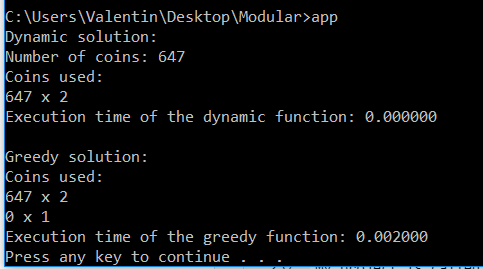
\includegraphics[scale=0.6]{gcc-1.png}
\\

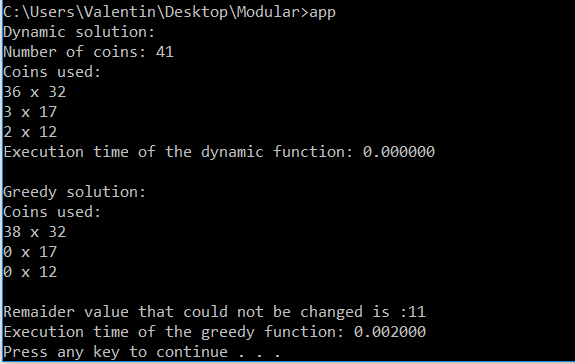
\includegraphics[scale=0.6]{gcc-2.png}
\\

\textcolor{red}{For a small input size the dynamic execution time is close to 0 seconds whereas the execution time for the greedy algorithm is countable.}\\

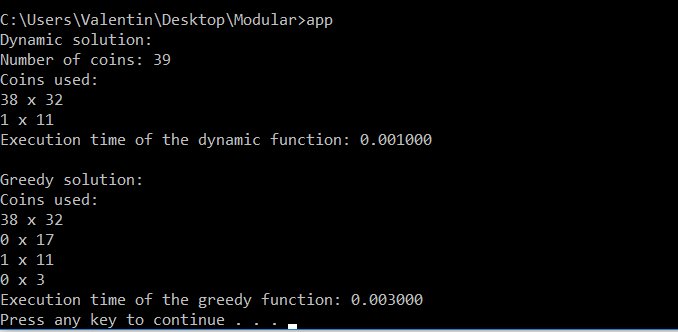
\includegraphics[scale=0.6]{gcc-3.png}\\

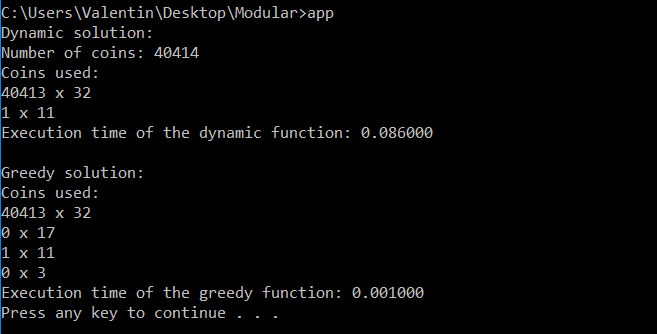
\includegraphics[scale=0.6]{gcc-4.png}\\

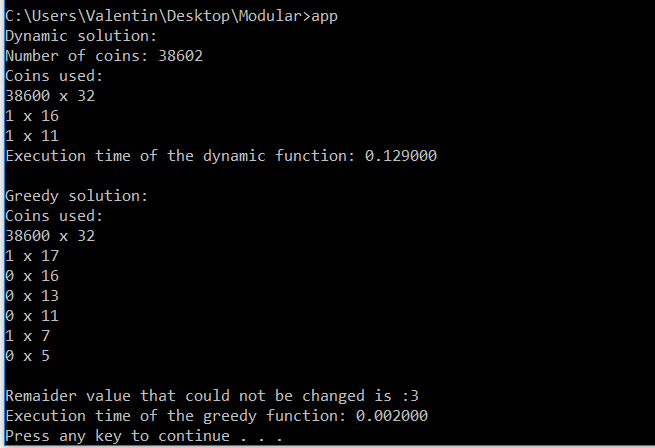
\includegraphics[scale=0.6]{gcc-5.png}\\


\textcolor{red}{For a big input size the dynamic execution time is higher than the execution time of the greedy approach as shown in the above pictures taken from different tests.}



\newpage
\section{Conclusion}
\textbf{}

This program depends on the size of the file , the dynamic approach has an execution time close to 0 for a small file but for a big file with a high owed sum and a high number of coins the execution time goes up by much .But using dynamic programming, the solution of the problem is always effective and optimal.

The greedy approach ,on the other hand,has a relatively constant execution time and it does not increase by much when the file gets larger . But its solution is not optimal every time.

The most challenging part of this program was the dynamic allocation of a matrix inside the dynamic implementation and also the method itself which is notably harder to comprehend with compared to the greedy method which is easy to use and understand but not as effective .


\newpage
\section{References}

\textbf{Books}:

1. Totul despre C si C++ 

Year of publication  :2005

Publisher :Teora

Author :Dr. Kris Jamsa Lars Klander\\
\textbf{Web references}:

$1.http://www.geeksforgeeks.org$

$2.https://www.sharelatex.com/learn/Main_Page$

$3.https://www.reddit.com/r/C_Programming$
\\
\textbf{Article}:

$1.https://en.wikipedia.org/wiki/Change-making\_problem$

\end{document}

